\documentclass[11pt]{article}

\usepackage{graphicx}
\usepackage{fancyhdr}
\setlength{\topmargin}{-.5in}
\setlength{\textheight}{9in}
\setlength{\oddsidemargin}{.125in}
\setlength{\textwidth}{6.25in}
\graphicspath{images/}
\begin{document}
\title{Robotics}
\author{Robert Game, Chris Johns, Tsz-Him Kwan, Paul Lowrie, Richard Sommerville}
\date{}
\maketitle

\section*{Braitenberg Behaviours}

Braitenberg behaviours are robots designed with actions that use a simple mapping of sensory information to motors to emulate basic organic behaviours. These were first put forward in 1984 by Braitenberg in his paper “Vehicles: Experiments in synthetic psychology" and are a way of emulating the actions of an animal in a natural environment. For this coursework we have implemented four behaviours, which are defined below:
\\
\\
For the general design of our Braitenberg behaviours we have used a general function \- executeBrait to map the E\-Puck's proximity sensors. In this function we first check the proximity sensors on the left (ps6 \& ps7) and right (ps0 \& ps1) to check if there are any objects directly in front of the robot. These values are combined to produce a value for information on the left and right of the robot \- this is then multiplied by BRAIT\_PROX\_OFFSET (0.75) which maps the sensor value directly to the capabilities of the stepper motors. At this point we have included a constant, BRAIT\_PROX\_THRESHOLD which accounts for noise on the sensors, this has been defined as 200 and prevents the robot from erroneously changing behaviour due to noise.

\begin{figure}[h]
\begin{center}
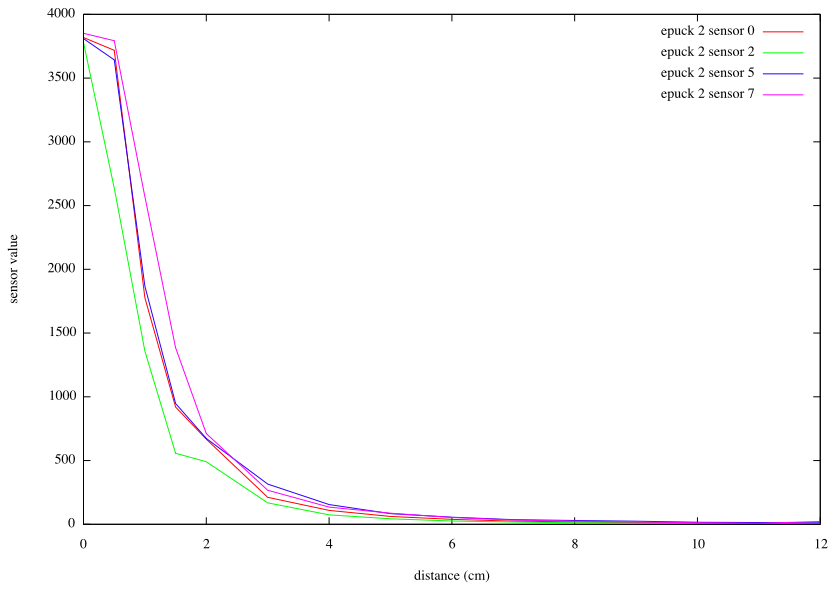
\includegraphics[width=0.5\textwidth]{epuck-2-proximity.png}
\caption{Sensor values to distance (Duarte, 2012)}
\end{center}
\end{figure}

If either of the sensors register a value above the noise threshold, prox0 (combined right sensor) and prox7 (combined left) will be doubled and passed through to the the defined behaviour. As a check, the sensor value will first ensure that the sensor mappings cannot exceed the maximum value for the motors - if they do this will be capped to the maximum speed we have defined for the stepper motor (900). If the sensors do not exceed the maximum it is then checked whether the speed is lower than the minimum we have defined for the motors (300) if it does not exceed this the speed is set to the minimum. At this point the values for each sensor, which have been mapped to an equivalent motor speed, are passed to the relevant behaviour function, this is done by storing the value of the E-Puck selector in a variable behaviour and checking it in a switch statement.

\subsection*{Aggression}

The aggression function takes the left and right sensor values as parameters, the function then maps the value of the right sensor to the left wheel, and the left sensor to the right wheel. This results in behaviour whereby an object in proximity to the right of the robot results in a sharp right turn, and an object in proximity to the left of the robot results in a sharp left turn. Due to the exponentially increasing value provided by the proximity sensor, the robot will also accelerate towards the stimuli, as defined in Braitenberg's paper.

\subsection*{Fear}

The fear behaviour acts in a similar manner to the aggression behaviour, however the values from the left sensors now map to the wheels on the same side. This results in the robot sharply turning away from the stimuli, as if afraid of it.

\subsection*{Curiosity}

As discussed in Braitenberg's book, the curious behaviour (Explorer) will be drawn to an object coming within a close proximity, however, unlike love (discussed below) the curious behaviour will continue to move. Eventually driving away from the object 'in order to find a more permanent and gratifying appeasement' Braitenberg (1984)
\\
\\
The implementation of this behaviour takes the values from the left and right sensors as before. However instead of binding the motor speed directly to the sensor value it instead subtracts the sensor value from the E-Puck's max speed. This inverts the behaviour of the E-Puck as it now slows down as the light source gets stronger as opposed to before when the E-Puck increased in speed as the light source gets stronger.

\subsection*{Love}

The Love behaviour is similar to the Curious behaviour in that the E-Puck slows down in speed as it is exposed to more light. However instead of driving away from the light source, the E-Puck stops and observes the object 'in quiet admiration from the time it spots the source to all future time' (Braitenberg, 1984). As the E-Puck approaches the object the speeds on the left and right motors are decreased as the sensor values increase. This happens until the sensor values increase to the point where they cancel out the motors, forcing the E-Puck to remain stationary.

\subsection*{Function Definitions}

\begin{itemize}
\item{executeBrait(): Collects sensor information and maps it to a motor speed. Select statement then chooses which behaviour to run.}
\item{aggression(): Maps the left motor speed to the right sensor and right to left - turning towards target}
\item{fear(): Maps the left sensor value to the left motor and right to right - turning away from target}
\item{love(): Subtracts the sensor value from the max speed of the motor. E-Puck eventually stops when numbers cancel}
\item{curious(): Subtracts the sensor value from the speed of the opposite motor. E-Puck slows down but begins to drive away from obstacle}
\end{itemize}

\section*{Obstacle Avoidance:}

The aim of this task was to implement an algorithm to allow the E-Puck to travel to a target location whilst avoiding obstacles along the way. 
\\
\\
The program comprises of two main behaviours: target seeking and obstacle avoidance. The target seeking section works using a defined X,Y plane, the E-Puck begins at point (0,0) and has a defined goal to drive towards - in our demo we used (0,50) which equates to 50cm in the Y axis.
\\
\\
Once the E-Puck has initiated it's location (0,0), it updates both it's current location and the orientation at a set interval. It does this using the UpdateCurrentPos() function, in this function the number of steps taken by each wheel is used to calculate the change in location and orientation of the E-Puck. This function finds the number of steps performed by each wheel since the previous update and uses this in conjunction with the MOTOR\_DIST constant to calculate the current angle and location of the E-Puck on the plane. The function then uses GetAngleWithinRange() to determine an equivalent angle within the range \begin{math}-\pi < angle \leq +\pi\end{math}
\\
\\
When navigation initiates, the E-Puck will determine the angle change required to face the target. This is calculated within GetAngleChange() where Pythagoras' theorem is used to calculate the angle between the current orientation and the orientation required to face the goal. The function returns an angle within the range \begin{math}-\pi < angle \leq +\pi\end{math} as well.
\\
\\
The E-Puck will begin turning left or right, depending on whether the angle returned is positive or negative. This ensures that the E-Puck takes the shortest route in order to orientate itself towards the target location. Once the E-Puck is facing an angle within the threshold of the target it will begin to drive towards it. This is done within the function MoveForwardsToTarget() which constantly checks if it has arrived within a threshold of the target destination, if it has it will stop the motors, if not, it will continue to drive forwards.
\\
\\
When the UpdateNav() function detects an obstacle in front of the E-Puck it will set a switch to initiate the obstacle avoidance behaviour. Once this is set, the E-Puck will circumnavigate the obstacle until it detects that it is once again facing it's target. Once this occurs it will travel forwards towards the goal.
\\
\\
While the E-Puck is hugging the wall and cannot see the target it will aim to keep the obstacle on it's left side. It uses the constant SENSOR\_WALL\_DIST to ensure that the wall is kept at a suitable distance. If the sensor detects that the object is no longer directly on it's left side, it then use the rear left sensor to ensure that it has fully cleared the object and has room to turn the corner. Once it has turned the corner it will continue to follow the wall until the E-Puck is orientated towards the goal, where it continues its target seeking behaviour.

\subsection*{Function Definition}

\begin{itemize}
\item{GetCurPosX(): returns current X coordinate}
\item{GetCurPosY(): returns current Y coordinate}
\item{GetCurAngle(): returns the current angle of the E-Puck}
\item{InitNavigation(): Initiates navigation and sets all starting values to 0}
\item{UpdateCurrentPos(): updates the current orientation and location of E-Puck}
\item{FollowLeftWall(): follows wall keeping left sensors within threshold}
\item{GetAngleWithinRange(): determines an equivalent angle in the range \begin{math}-\pi < angle \leq +\pi\end{math}}
\item{GetAngleChange(): calculates the angle change required in order to face target}
\item{StartTurning(): sets the E-Puck to turn left or right based on the angle}
\item{SetTarget(): sets the target location in terms of X,Y values}
\item{SetTargetInCM(): sets the target location in terms of cm}
\item{UpdateNav(): checks current state of the E-Puck and calls correct function based on its state}
\item{TurnToTarget(): checks whether the current turn has completed, if it hasn't it continues the turn}
\item{MoveForwardsToTarget(): checks whether the E-Puck is at it's target, if it it then stops the motors. If not, it begins to turn}
\item{SwitchLED(param1, param2): switches the LED defined in param1 using param2. For example (3,1) would turn LED3 on. If param1 = -1 it turns all LEDs on}
\end{itemize}

\pagebreak

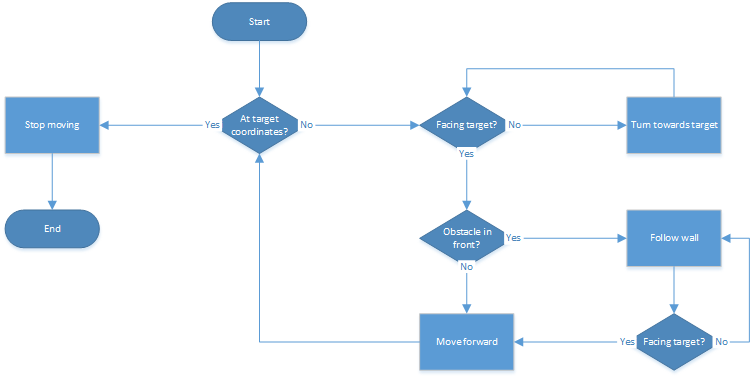
\includegraphics[width=1.5\textwidth, angle=-90]{ObstacleAvoidance.png}

\section*{High Level Behaviour: Zombie Infection}

For our high level behaviour we have implemented a zombie infection simulation. In this we have used multiple E-Pucks in order to show the spread of a Zombie Virus. The E-Puck can take two different forms in this, a Human or a Zombie. For our demonstration we release one zombie into a box containing multiple humans E-Pucks. The Zombie will eventually find and infect the other E-Pucks.
\\
\\
A standard E-Puck will begin as a human. In this state the E-Puck will drive forward until one of the sensors detects that an obstacle is closer than ZOMBIE\_WALL\_DIST (700), in which case it will turn away from the obstacle and continue to drive forward. 
\\
\\
In the Zombie behaviour, all of the LEDs on the E-Puck will be illuminated to distinguish them from humans and also to provide a light source used to determine whether infection occurs. The Zombie will drive forwards while initiating the Braitenberg Aggression behaviour defined earlier. This means that the Zombie will attack any and all obstacles it sees. When either front sensor values have hit a threshold to indicate that it has successfully attacked the obstacle, defined by HIT\_THRESHOLD, a random value between the range of  \begin{math}\pi \pm \frac{\pi}{6}\end{math} is calculated and added to the current orientation angle and set as the target (This angle is once again converted to a value within the range of \begin{math}-\pi < angle \leq +\pi\end{math} using the GetAngleWithinRange() function) to turn the Zombie around. A random value is used to add arbitrary behaviour to the Zombie.
\\
\\
The human behaviour loops through it's proximity sensors and continually checks the readings from each as it travels. A value higher than ZOMBIE\_WALL\_DIST is assumed to be an obstacle and the E-Puck will begin to turn away from it as described above. As an obstacle is assumed to be stationary the E-Puck will never trigger the Zombie behaviour as it will have avoided the obstacle before HIT\_THRESHOLD (1250) is reached. In contrast, an attacking Zombie will have triggered its aggressive behaviour as the E-Pucks pass, forcing the values past the HIT\_TRESHOLD and infecting the Human. The Zombie uses the larger front LED to provide extra light in order to ensure that this threshold is breached and the infection can occur. When the human E-Puck senses that the infection is successful it executes its Zombie behaviours. At this point they drive away from each other and continue to execute Braitenberg's Aggressive behaviour

\subsection*{Function Definitions}

\begin{itemize}
\item{isHuman(): returns whether the E-Puck is human or not}
\item{executeHuman(): checks whether there it has been hit, changes to Zombie if it has. Otherwise continues to run away}
\item{executeZombie(): turns all LEDs on. If Zombie is not turning, checks whether it has hit anything, if it has begins to turn. If not continues to be aggressive. If state is turning and it has turned within threshold it stops turning}
\end{itemize}

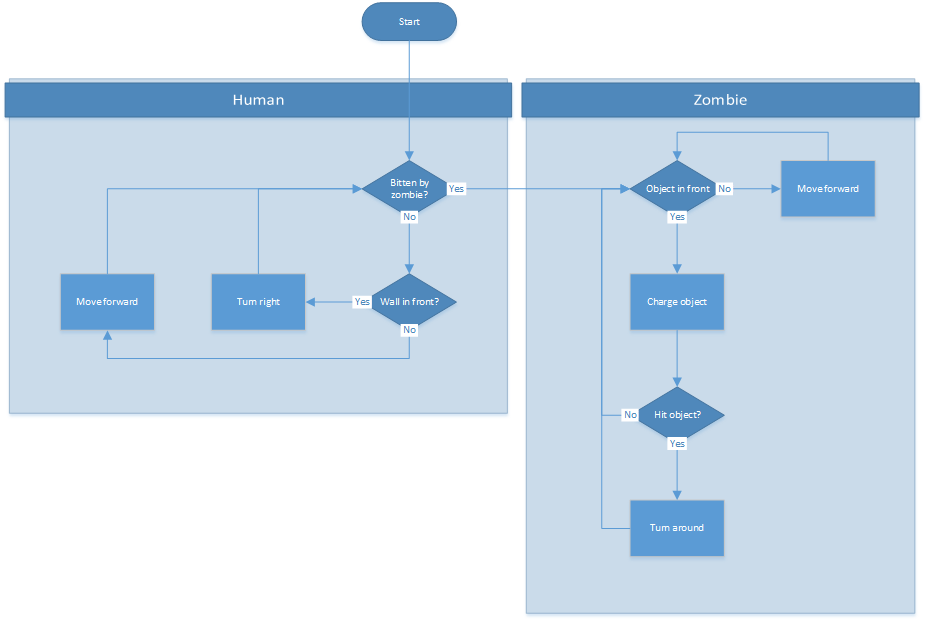
\includegraphics[width=1.4\textwidth, angle=-90]{ZombieInfection.png}

\section*{Test Plans}

\subsection*{Braitenberg Aggression:}


\begin{center}
\begin{tabular}{ | p{5cm} | p{5cm} | p{5cm} |}
	\hline
	\textbf{Situation} & \textbf{Expected Behaviour} & \textbf{Actual Behaviour} \\
    \hline
	Obstacle in front & Drive towards obstacle increasing speed up to max & As expected \\
	\hline
	Obstacle front left & Turn toward obstacle increasing speed up to max & As expected \\
	\hline
	Obstacle front right & Turn toward obstacle increasing speed up to max & As expected \\
	\hline
\end{tabular}
\end{center}

\subsection*{Braitenberg Fear:}

\begin{center}
\begin{tabular}{ | p{5cm} | p{5cm} | p{5cm} |}
	\hline
	\textbf{Situation} & \textbf{Expected Behaviour} & \textbf{Actual Behaviour} \\
    \hline
	Obstacle in front & Turn away from obstacle increasing speed  & As expected \\
	\hline
	Obstacle front left & Turn away from obstacle increasing speed  & As expected \\
	\hline
	Obstacle front right & Turn away from obstacle increasing speed  & As expected \\
	\hline
\end{tabular}
\end{center}

\subsection*{Braitenberg Love:}

\begin{center}
\begin{tabular}{ | p{5cm} | p{5cm} | p{5cm} |}
	\hline
	\textbf{Situation} & \textbf{Expected Behaviour} & \textbf{Actual Behaviour} \\
    \hline
	Obstacle in front & Drive towards obstacle reducing speed and stop directly in front  & As expected \\
	\hline
	Obstacle front left & Drive towards obstacle reducing speed and stop directly in front  & As expected \\
	\hline
	Obstacle front right & Drive towards obstacle reducing speed and stop directly in front  & As expected \\
	\hline
\end{tabular}
\end{center}

\subsection*{Braitenberg Curiosity:}

\begin{center}
\begin{tabular}{ | p{5cm} | p{5cm} | p{5cm} |}
	\hline
	\textbf{Situation} & \textbf{Expected Behaviour} & \textbf{Actual Behaviour} \\
    \hline
	Obstacle in front & Turn away from obstacle reducing speed and return to normal speed when obstacle not present  & As expected \\
	\hline
	Obstacle front left & Turn away from obstacle reducing speed and return to normal speed when obstacle not present  & As expected \\
	\hline
	Obstacle front right & Turn away from obstacle reducing speed and return to normal speed when obstacle not present  & As expected \\
	\hline
\end{tabular}
\end{center}

\subsection*{Path Finding + Obstacle Avoidance}

 \begin{center}
\begin{tabular}{ | p{5cm} | p{5cm} | p{5cm} |}
	\hline
	\textbf{Situation} & \textbf{Expected Behaviour} & \textbf{Actual Behaviour} \\
    \hline
	Clear path & Turns to target and moves directly to it & As expected \\
	\hline
	Flat obstacle in path & Once obstacle is met, turns right and follows wall until clear path to target is seen & As expected \\
	\hline
	Round obstacle in path & Once obstacle is met, turns right and follows wall until clear path to target is seen & As 	expected \\
	\hline
	Multiple obstacles in path & Once obstacle is met, turns right and follows wall until clear path to target is seen & As expected\\
	\hline
\end{tabular}
\end{center}

\subsection*{Zombie Infection}

 \begin{center}
\begin{tabular}{ | p{5cm} | p{5cm} | p{5cm} |}
	\hline
	\textbf{Situation} & \textbf{Expected Behaviour} & \textbf{Actual Behaviour} \\
    \hline
	Human with clear path & Moves forward & As expected \\
	\hline
	Human with obstacle in path & Once obstacle is met, turns away & As expected \\
	\hline 
	Human hit by Zombie & All LEDs lit, gets infected & As expected \\
	\hline 
	Zombie with clear path & Moves forward &As expected \\
	\hline 
	Zombie with obstacle in path & Drive towards obstacle increasing speed up to max & As expected \\
	\hline 
	Zombie hits Human & Hit detected, turns at random angle & As expected \\
	\hline 
	Zombie hits Zombie & Hit detected, turns at random angle & As expected \\
	\hline 
	Zombie hits wall & Hit detected, turns at random angle & As expected \\
	\hline 
\end{tabular}
\end{center}

\section*{References}

\begin{enumerate}
\item{Miguel Duarte (2012), A quick analysis of the e-puck's infrared proximity and light sensors, Viewed 11/12/14, http://miguelduarte.pt/2012/03/26/an-analysis-of-the-e-pucks-infrared-proximity-sensors/}
\item{Valentino Braitenberg (1984), Vehicles: Experiments in Synthetic Psychology, MIT Press}
\end{enumerate}

\end{document}
